\documentclass[11pt,letterpaper]{article}
\usepackage[top=3cm, bottom=2cm, left=2cm, right=2cm, columnsep=20pt]{geometry}
\usepackage{pdfpages}
\usepackage{graphicx}
\usepackage{etoolbox}
\apptocmd{\sloppy}{\hbadness 10000\relax}{}{}
% \usepackage[numbers]{natbib}
\usepackage[T1]{fontenc}
\usepackage{ragged2e}
\usepackage[french]{babel}
\usepackage{listings}
\usepackage{color}
\usepackage{soul}
\usepackage[utf8]{inputenc}
\usepackage[export]{adjustbox}
\usepackage{caption}
\usepackage{amsmath}
\usepackage{amssymb}
\usepackage{float}
\usepackage{csquotes}
\usepackage{fancyhdr}
\usepackage{wallpaper}
\usepackage{siunitx}
\usepackage[indent]{parskip}
\usepackage{textcomp}
\usepackage{gensymb}
\usepackage{multirow}
\usepackage[hidelinks]{hyperref}
\usepackage{abstract}
\renewcommand{\abstractnamefont}{\normalfont\bfseries}
\renewcommand{\abstracttextfont}{\normalfont\itshape}
\usepackage{titlesec}
\titleformat{\section}{\large\bfseries}{\thesection}{1em}{}
\titleformat{\subsection}{\normalsize\bfseries}{\thesubsection}{1em}{}
\titleformat{\subsubsection}{\normalsize\bfseries}{\thesubsubsection}{1em}{}

\usepackage{xcolor}
\definecolor{codegreen}{rgb}{0,0.6,0}
\definecolor{codegray}{rgb}{0.5,0.5,0.5}
\definecolor{codepurple}{rgb}{0.58,0,0.82}
\definecolor{backcolour}{rgb}{0.95,0.95,0.92}
\lstdefinestyle{mystyle}{
    backgroundcolor=\color{backcolour},   
    commentstyle=\color{codegreen},
    keywordstyle=\color{magenta},
    numberstyle=\tiny\color{codegray},
    stringstyle=\color{codepurple},
    basicstyle=\ttfamily\footnotesize,
    breakatwhitespace=false,         
    breaklines=true,                 
    captionpos=b,                    
    keepspaces=true,                 
    numbers=left,                    
    numbersep=5pt,                  
    showspaces=false,                
    showstringspaces=false,
    showtabs=false,                  
    tabsize=2
}
\lstset{style=mystyle}

\usepackage[most]{tcolorbox}
\newtcolorbox{note}[1][]{
  enhanced jigsaw,
  borderline west={2pt}{0pt}{black},
  sharp corners,
  boxrule=0pt, 
  fonttitle={\large\bfseries},
  coltitle={black},
  title={Note:\ },
  attach title to upper,
  #1
}

%----------------------------------------------------

\setlength{\parindent}{0pt}
\DeclareCaptionLabelFormat{mycaptionlabel}{#1 #2}
\captionsetup[figure]{labelsep=colon}
\captionsetup{labelformat=mycaptionlabel}
\captionsetup[figure]{name={Figure }}
\newcommand{\inlinecode}{\normalfont\texttt}
\usepackage{enumitem}
\setlist[itemize]{label=\textbullet}

\begin{document}
\begin{titlepage}
\center

\begin{figure}
    \ThisULCornerWallPaper{.4}{Polytechnique_signature-RGB-gauche_FR.png}
\end{figure}
\vspace*{2 cm}

\textsc{\Large \textbf{PHS2223 --} Introduction à l'optique moderne}\\[0.5cm]
\large{\textbf{Équipe : 04}}\\[1.5cm]

\rule{\linewidth}{0.5mm} \\[0.5cm]
\Large{\textbf{Expérience 1}} \\[0.2cm]
\text{Microscopie confocale}\\
\rule{\linewidth}{0.2mm} \\[2.3cm]

\large{\textbf{Présenté à}\\
  Guillaume Sheehy\\
  Esmat Zamani\\[2.5cm]
  \textbf{Par :}\\
  Émile \textbf{Guertin-Picard} (2208363)\\
  Laura-Li \textbf{Gilbert} (???????)\\
  Tom \textbf{Dessauvages} (???????)\\[3cm]}

\large{\today\\
Département de Génie Physique\\
Polytechnique Montréal\\}

\end{titlepage}

%----------------------------------------------------

\tableofcontents
\pagenumbering{roman}
\newpage

\pagestyle{fancy}
\setlength{\headheight}{14pt}
\renewcommand{\headrulewidth}{0pt}
\fancyfoot[R]{\thepage}

\pagestyle{fancy}
\fancyhf{}
\renewcommand{\headrulewidth}{1pt}
\fancyhead[L]{\textbf{PHS2223}}
\fancyhead[C]{Microscopie confocale}
\fancyhead[R]{\today}
\fancyfoot[R]{\thepage}

\pagenumbering{arabic}
\setcounter{page}{1}

%----------------------------------------------------

\section{Introduction}

\section{Théorie}
\subsection{Microsopie Confocale}
La microscopie confocale est une technique d'imagerie avancée qui permet l'obtention d'images à hautes résolution, en éliminant la lumière hors-focus, particulièrement ceux à l'extérieur du plan focal. Le fonctionnement de cette technologie repose sur les principes d'illumination et de détection limités à un certain volume par la présence d'un simple trou, nommé sténopé (Source 1). En d'autres termes, une source de lumière, telle qu'un laser, est émise à travers le système, celle-ci est, ensuite, dirigée vers des miroirs dichroïques qui permettent la sélection de certaines longueurs d'onde réfléchies (Source 2). Une fois redirigée, la lumière réfléchie par les miroirs passe à travers une première lentille, concentrant ainsi le faisceau en un point précis, soit l'objet. Une fois arrivée à l'échantillon, une partie de ce faisceau est réfléchi par l'objet et, par le fait même, retransmis vers les miroirs. La lumière provenant de l'échantillon est alors redirigée vers le sténopé, situé derrière une deuxième lentille qui permet la convergence du rayon lumineux. Celle-ci traverse, ensuite, le sténopé, petite ouverture permettant d'éliminer les faisceaux ne provenant pas du plan focal, et atteint le détecteur. Puisque l'oeil nu n'est pas en mesure de traiter l'image résultante, le détecteur reconstruit indirectement l'image à l'aide de balayages de l'échantillon. De cette manière, le faisceau se déplace, selon les différentes positions axiales, sur l'objet afin d'obtenir une image complète (Source 3).

% Source 1 : chrome-extension://efaidnbmnnnibpcajpcglclefindmkaj/https://sfa.univ-poitiers.fr/imageup/wp-content/uploads/sites/31/2014/06/Principe_Confocal-2.pdf
% Source 2 : https://chineselens.com/fr/dichroic-mirrors/
% Source 3 : Procédurier

\section{Méthodologie}

\section{Hypothèses}

\begin{figure}[H]
  \centering
  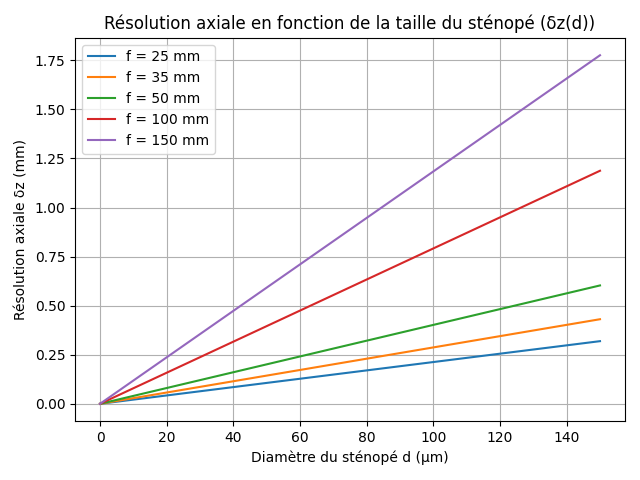
\includegraphics[scale=0.6]{res_vs_pinhole.png}
  \caption{test}
  \label{respin}
\end{figure}

\begin{figure}[H]
  \centering
  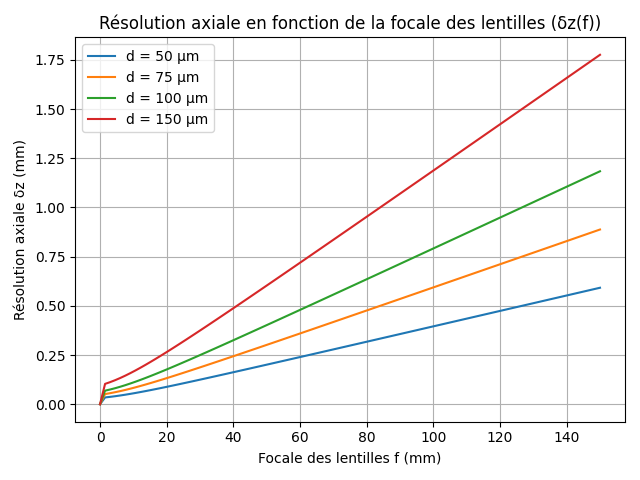
\includegraphics[scale=0.6]{res_vs_focal.png}
  \caption{test}
  \label{resfoc}
\end{figure}

\begin{figure}[H]
  \centering
  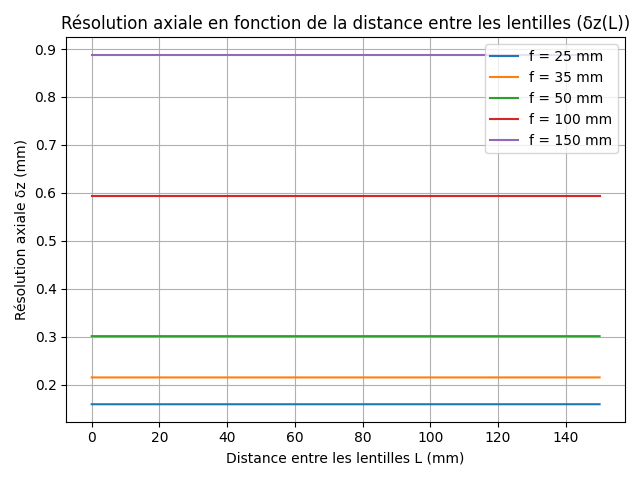
\includegraphics[scale=0.6]{res_vs_L.png}
  \caption{test}
  \label{resl}
\end{figure}



\section{Annexes}

\subsection{Modèle mathématique pour la simulation}



\subsection{Code source}



\clearpage

% \bibliographystyle{unsrtnat}
% \bibliography{My_Library}

\end{document}
